\documentclass[11pt,compress,t,notes=noshow, aspectratio=169, xcolor=table,dvipsnames]{beamer}

\usepackage{../../style/lmu-lecture}

% %  New colors
\definecolor{ggRed}{HTML}{F8766D}
\definecolor{ggGreen}{HTML}{00BFC4}
\definecolor{rep}{HTML}{3646f1}
\definecolor{cice}{HTML}{00BFFF}
\definecolor{mygreen}{HTML}{0FA90F}
\definecolor{amber}{rgb}{0.9, 0.7, 0.1}

\newcommand{\highlightICE}[1]{\colorbox{cice}{$\displaystyle #1$}}
\newcommand{\highlight}[1]{\colorbox{orange}{$\displaystyle #1$}}
\newcommand{\highlightYG}[1]{\colorbox{YellowGreen!50}{$\displaystyle #1$}}
\newcommand{\highlightFG}[1]{\colorbox{ForestGreen!70}{$\displaystyle #1$}}

\usepackage{tikz}
\usetikzlibrary{shapes,arrows,automata,positioning,calc,chains,trees, shadows}
\tikzset{
  %Define standard arrow tip
  >=stealth',
  %Define style for boxes
  punkt/.style={
    rectangle,
    rounded corners,
    draw=black, very thick,
    text width=6.5em,
    minimum height=2em,
    text centered},
  % Define arrow style
  pil/.style={
    ->,
    thick,
    shorten <=2pt,
    shorten >=2pt,}
}

% definition of the style
\tikzset{exampleblock/.style={rounded corners,rectangle split, rectangle split parts=4, draw, 
rectangle split part fill={gray!20, gray!20, cice!20, orange!20},minimum width=0.3\textwidth
}}
\tikzset{main node/.style={rectangle,draw,minimum size=1cm,inner sep=4pt},}
\usetikzlibrary{calc}
\usetikzlibrary{chains, positioning, arrows, trees, shadows}
%\input{figure/gear.tex}
%http://tex.stackexchange.com/questions/6135/how-to-make-beamer-overlays-with-tikz-node
\tikzset{
  %Style of the black box
  bbox/.style={draw, fill=black, minimum size=3cm,
  label={[white, yshift=-1.3em]above:$in$},
  label={[white, yshift=1.3em]below:$out$},
  label={[rotate = 90, xshift=1em, yshift=0.5em]left:Black-Box}
  },
  multiple/.style={double copy shadow={shadow xshift=1.5ex,shadow
  yshift=-0.5ex,draw=black!30,fill=white}},
}

% for overlay box
\usetikzlibrary{backgrounds,shapes.multipart}
\pgfdeclarelayer{myback}
\pgfsetlayers{background,main,myback} %<= insert the myback 
% after the "main" to display the content in front of the usual content


% Defines macros and environments
% This file is included in slides and exercises

% Rarely used fontstyle for R packages, used only in 
% - forests/slides-forests-benchmark.tex
% - exercises/single-exercises/methods_l_1.Rnw
% - slides/cart/attic/slides_extra_trees.Rnw
\newcommand{\pkg}[1]{{\fontseries{b}\selectfont #1}}

% Spacing helpers, used often (mostly in exercises for \dlz)
\newcommand{\lz}{\vspace{0.5cm}} % vertical space (used often in slides)
\newcommand{\dlz}{\vspace{1cm}}  % double vertical space (used often in exercises, never in slides)
\newcommand{\oneliner}[1] % Oneliner for important statements, used e.g. in iml, algods
{\begin{block}{}\begin{center}\begin{Large}#1\end{Large}\end{center}\end{block}}

% Don't know if this is used or needed, remove?
% textcolor that works in mathmode
% https://tex.stackexchange.com/a/261480
% Used e.g. in forests/slides-forests-bagging.tex
% [...] \textcolor{blue}{\tfrac{1}{M}\sum^M_{m} [...]
% \makeatletter
% \renewcommand*{\@textcolor}[3]{%
%   \protect\leavevmode
%   \begingroup
%     \color#1{#2}#3%
%   \endgroup
% }
% \makeatother


\title{Interpretable Machine Learning}
% \author{LMU}
%\institute{\href{https://compstat-lmu.github.io/lecture_iml/}{compstat-lmu.github.io/lecture\_iml}}
\date{}

\begin{document}

\newcommand{\titlefigure}{figure/ale_plot.pdf}
\newcommand{\learninggoals}{
\item Difference between feature effects and feature interactions
\item REPID
}

\lecturechapter{Regional Effects}
\lecture{Interpretable Machine Learning}


\begin{frame}
  \frametitle{Recap: Local/Global explanations}
  \begin{itemize}
    \item Global explanations (e. g. PD plot)
    \begin{itemize}
      \item \textbf{Pro}: Universal explanation (applies to the whole model)
      \item \textbf{Con}: Oversimplify, lack fidelity
      \item \textbf{Con}: Can produce misleading explanations when feature interactions are present 
    \end{itemize}
    \item Local explanations (e. g. ICE curves, Shapley values)
    \begin{itemize}
      \item \textbf{Pro}: Precise explanations
      \item \textbf{Con}: Limited to individual instances (not the whole model)
    \end{itemize}
  \end{itemize}
\end{frame}


\begin{frame}{Why regional explanations?}
    \textbf{Question:} How to produce plots in which feature effects are less confounded by interactions? \\
    \textbf{Idea:} Regional effect plots (REPs): Group homogeneous ICE curves in such a way that reduces the presence of individual interaction effects within a group.
  \noindent\makebox[\linewidth]{\rule{\paperwidth}{0.4pt}}
  \begin{columns}
      \column{0.33\textwidth}
      \centering
      \textbf{Global Effect}
      \begin{figure}
          \centering
          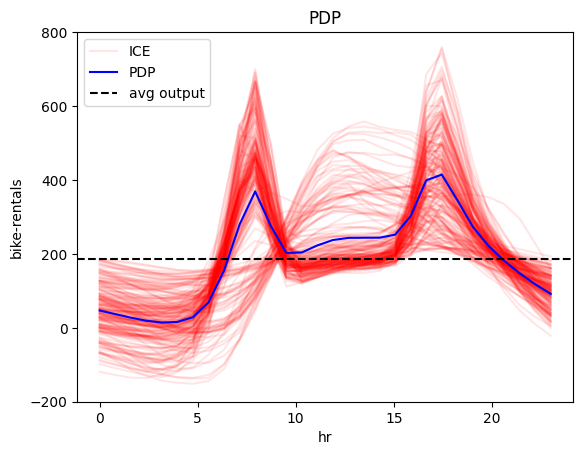
\includegraphics[width=.9\linewidth]{figure/01_bike_sharing_dataset_18_1.png}
      \end{figure}

      \hspace{2.5cm} % Horizontal spacing before the line      
      \column{0.33\textwidth}
      \centering
      \textbf{Regional Effect (1)}
        \begin{figure}
          \centering
          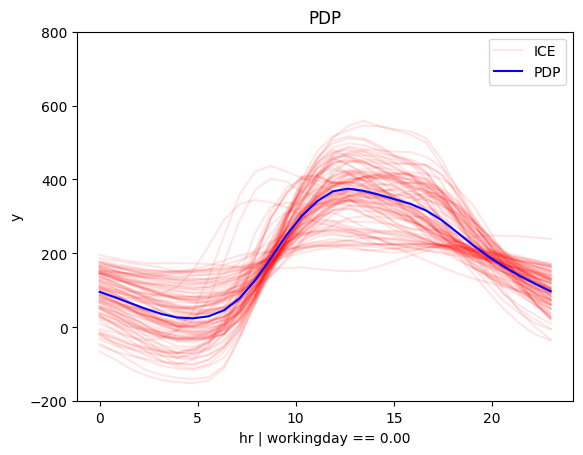
\includegraphics[width=.9\linewidth]{figure/01_bike_sharing_dataset_28_0.png}
      \end{figure}

     \column{0.33\textwidth}
     \centering
      \textbf{Regional Effect (2)}
        \begin{figure}
          \centering
          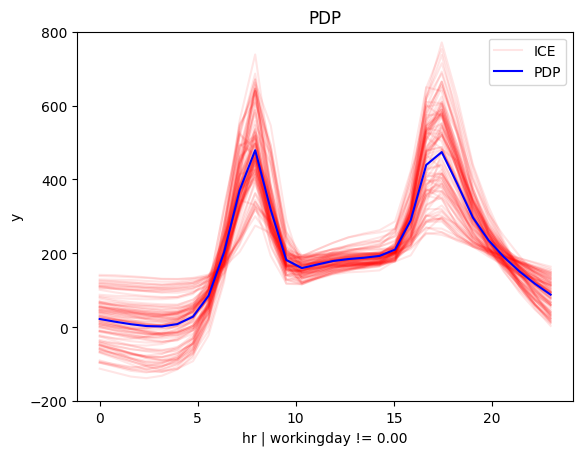
\includegraphics[width=.9\linewidth]{figure/01_bike_sharing_dataset_28_1.png}
      \end{figure}     
  \end{columns}
      \begin{itemize}
      \item Splitting by the "workingday" revealed 2 different patterns that we're clashed together in the initial plot
      \item $\cup_i (\texttt{regional\_explanation}_i) = \texttt{global\_explanation} $
      \item $Fidelity (\texttt{regional\_explanation}_i ) > Fidelity(\texttt{global\_explanation} ) $
      \end{itemize}
      
\end{frame}


\begin{frame}{ICE Curve: Local Feature Effects for ML Models}
%ICE curves show how different feature values of an observation affect its model prediction \newline $\Rightarrow$ \textbf{local interpretation method}
%From a local perspective, one might be interested in how changing feature values of an observation affect model prediction

\textbf{Question:} How do changes of feature values affect model prediction for a \textbf{single observation}?

%\smallskip

%\textbf{Idea:} Change values of observation and feature of interest, and visualize how prediction changes

% \textbf{Idea:} For each observation $\xv$, define individual conditional expectation $\fh({\color{red}\tilde x_j}, \xv_{-j})$ %ICE_j^\xv(\tilde x_j) := 
% \begin{itemize}
%     \item Partition $\xv = (x_j, \xv_{-j})$ into $x_j$ (feature of interest) and $\xv_{-j}$ (remaining features)
%     \item Replace observed value $x_j$ with {\color{red} grid values $\tilde x_j$} while keeping values $\xv_{-j}$ fixed
% \end{itemize}
\textbf{Idea:} Partition obs. $\xv = (x_j, \xv_{-j})$ into $x_j$ (feature of interest) and $\xv_{-j}$ (remaining features) 
\begin{itemize}
    \item Replace observed value $x_j$ with {\color{red} grid values $\tilde x_j$} while keeping values $\xv_{-j}$ fixed
    \item Visualize function $\fh({\color{red}\tilde x_j}, \xv_{-j})$ for varying ${\color{red}\tilde x_j}$ (individual conditional expectation, ICE)%ICE_j^\xv(\tilde x_j) := 
\end{itemize}

\pause

\textbf{Example:} Prediction surface of a SVM model (left), select observation and visualize changes in prediction for different values of $x_2$ while keeping $x_1$ fixed $\Rightarrow$ \textbf{local interpretation}

\vfill
\centering
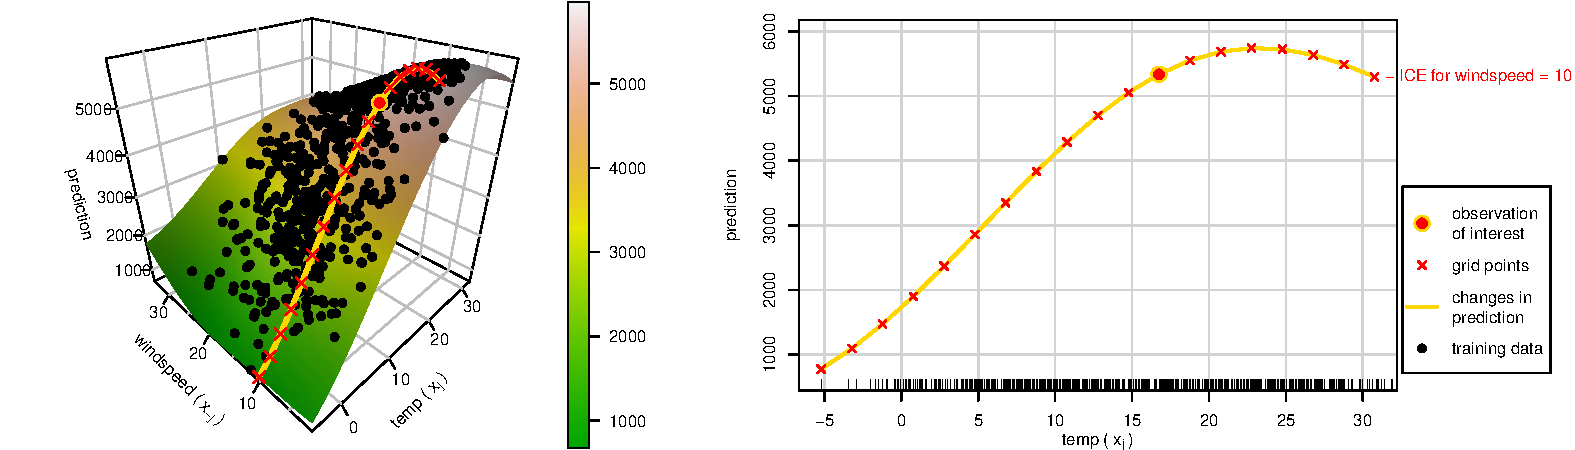
\includegraphics[width=0.95\textwidth, page = 1]{figure/ice_motivation_bike}

%$\Rightarrow$ Repeat for all observations and average the curves for global feature effect ($\leadsto$ PD plots)
\end{frame}



\begin{frame}{PD Plot - Global Feature Effects for ML Models}

\textbf{Question:} How do changes of feature values affect model prediction \textbf{on average}?

%\textbf{Idea:} 

\begin{itemize}
    \item \textbf{PD function}: Integrate out effect of $X_{-j}$ to obtain marginal effect of feature $x_j$
    
    \medskip
    
    \centerline{$ \textstyle
    f_j^{PD}(\tilde x_j) = \E_{X_{-j}}[\hat f(\tilde x_j, X_{-j})] = \int \hat f(\tilde x_j, X_{-j}) d \mathbb{P}(X_{-j})
    $}
        %with $C = S^\complement$. 

    \smallskip
    
    \item \textbf{Estimate (MC integration):} Average ICE curves at grid points $\tilde x_j$
    
    \medskip
    
    \centerline{$ \textstyle
    \hat f_j^{PD}(\tilde x_j) = \frac{1}{n} \sum_{i=1}^{n} \hat f(\tilde x_j, \xv_{-j}^{(i)})
    $}
\end{itemize}


\vfill
\centering
\includegraphics[width=0.95\textwidth, page = 2]{figure/ice_motivation_bike}

%Aggregates to Global PD
%point-wise average of ICE
%Extrapolation?
\end{frame}



\begin{frame}{Feature Interactions}

\textbf{Hooker (2004, 2007):} Functional ANOVA decomposition of a (prediction) function% into main and higher-order (interaction) effects

\begin{center}
    $\textstyle
\hat{f}(\mathbf{x}) = g_0 + 
\underbrace{\textstyle\sum_{j=1}^{p} {{g_j(x_j)}}}_{\text{{main effect}}} + 
\underbrace{\textstyle\sum_{j \neq k} {\textcolor{blue}{g_{j,k}(x_j, x_k)}}}_{\text{\textcolor{blue}{two-way interaction effect}}} + 
\cdots + 
\underbrace{{\textcolor{blue}{g_{1,2,\ldots,p}(\mathbf{x})}}}_{\text{\textcolor{blue}{p-way interaction effect}}}
$
\end{center}

%A function $f(\xv)$ is said to exhibit an interaction between two of its variables $x_j$ and $x_k$ if the difference in the value of $f(\xv)$ as a result of changing the value of $x_j$ depends on the value of $x_k$. For numeric variables, this can be expressed as
\textbf{Friedman and Popescu (2008):} %From functional ANOVA decomposition it follows
%A function $f(\xv)$ contains an interaction between $x_j$ and $x_k$ if a change in $f(\xv)$-values due to variations in $x_j$ also depend on $x_k$, i.e.: %, for numeric features:

%\medskip

%\centerline{$\mathbb{E} \left[ \tfrac{\partial^2 f(\xv)}{\partial x_j \partial x_k} \right]^2 > 0$}

%\medskip
\begin{itemize}
%is a sum of two functions, each independent of $x_j$, $x_k$:
% $f_{-j}$ and $f_{-k}$ that do not depend on $x_j$ and $x_k$, respectively:
    \item[$\Rightarrow$] If $x_j$ and $\xv_{-j}$ do not interact, we can decompose $f(\xv) = g_{j}(x_{j}) + g_{-j}(\xv_{-j})$
    \item[$\Rightarrow$] If $x_j$ and $x_k$ do not interact, we can decompose $f(\xv) = g_{-j}(\xv_{-j}) + g_{-k}(\xv_{-k})$
    %\item<3>[$\Rightarrow$] $\highlight{f(\xv) - g_{j}(x_{j}) - g_{-j}(\xv_{-j})} = 0$ %if there are no interactions between feature $j$ and any other feature $-j$
\end{itemize}


%\medskip

%\centerline{$f(\xv) = f_{-j}(x_1, \ldots, x_{j-1}, x_{j+1}, \ldots, x_p) + f_{-k}(x_1, \ldots, x_{k-1}, x_{k+1}, \ldots, x_p)$}


\only<1>{
{
\textbf{Example:} Not additively separable: \\
{\footnotesize $f(\xv) = x_1 + x_2 + x_1 \cdot x_2 \neq g(x_1) + g(x_2)$}

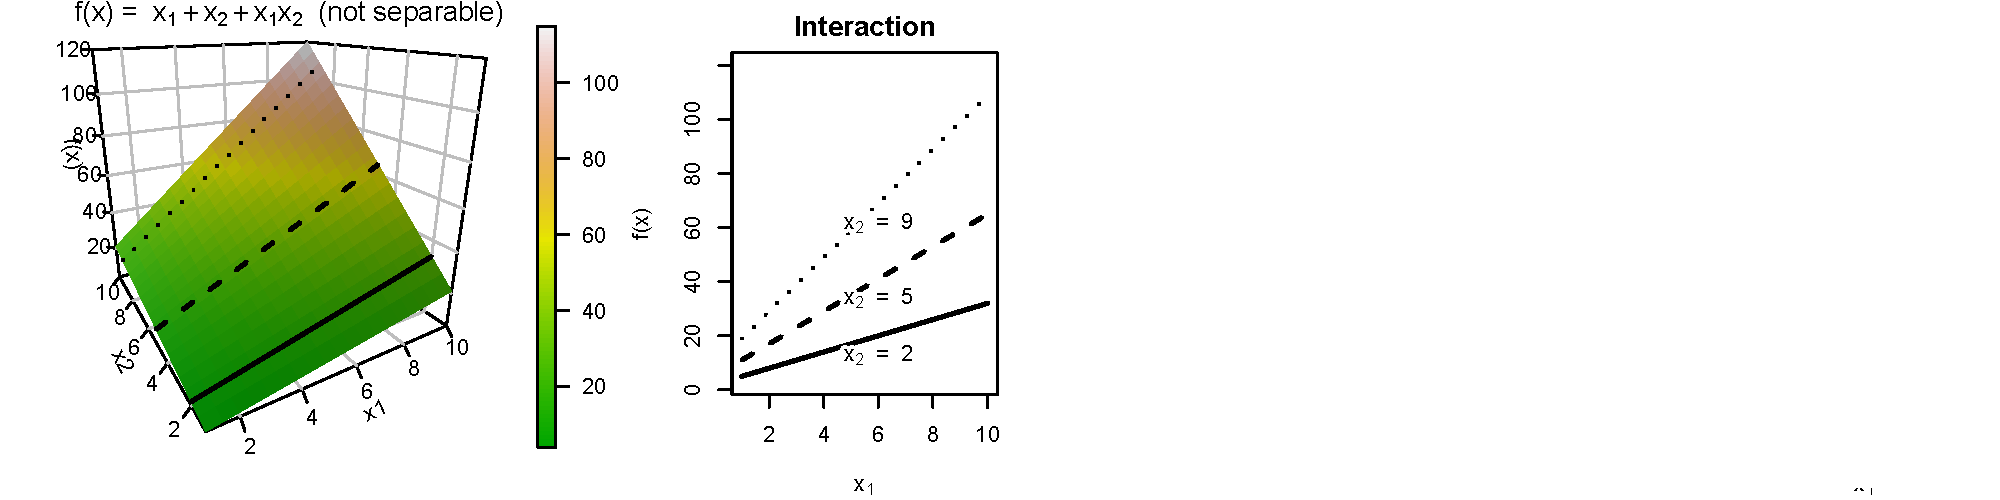
\includegraphics[width = 0.9\textwidth]{figure/interaction_separable_3}}
}
\only<2>{\textbf{Example:} Separable: {\footnotesize $f(\xv) = x_1 + x_2 + \log(x_1 \cdot x_2)
 	       = \left(x_1 + \log(x_1)\right) + \left(x_2 + \log(x_2)\right) = g_1(x_1) + g_2(x_2)$}
% \begin{itemize}
%     \item Not separable: $f(\xv) = x_1 + x_2 + x_1 \cdot x_2$
%     \item Separable: {\small $f(\xv) = x_1 + x_2 + \log(x_1 \cdot x_2)
% 	       = x_1 + \log(x_1) + x_2 + \log(x_2) = g_1(x_1) + g_2(x_2)$}
% \end{itemize}

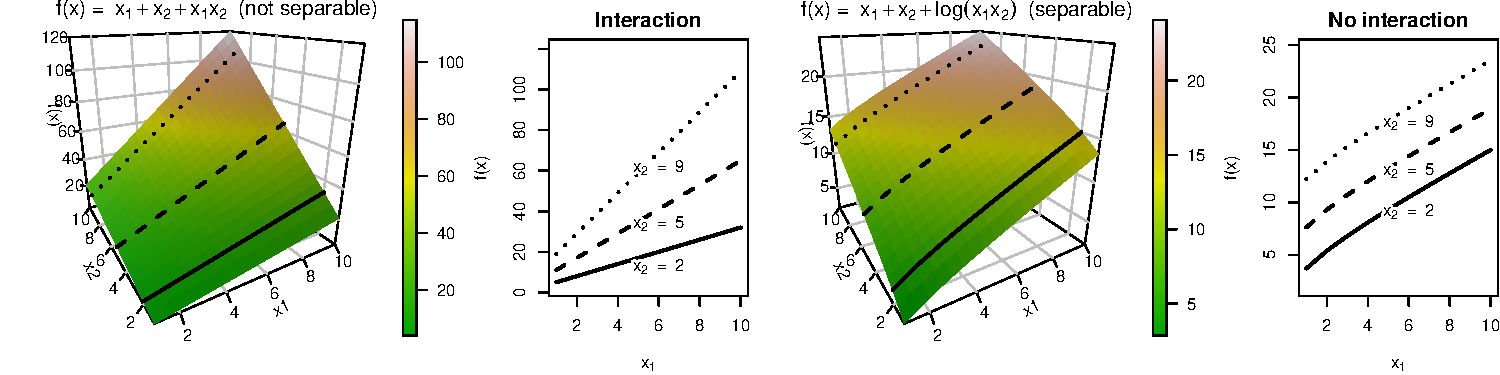
\includegraphics[width = 0.9\textwidth]{figure/interaction_separable_2}
%\pause\color{red}
%$\Rightarrow$ \textbf{Different shapes of ICE curves indicate interactions}
% ICE curves can be used to identify potential interactions (different shapes)
}
% \only<3>{

% \textbf{H-statistic:}

% The more $f^{PD,c}_{j}(x_j) + f^{PD,c}_{k}(x_k)$ deviates from $f_{j,k}^{PD,c}(\xv_{j,k})$, the stronger they interact:
% %The stronger a pair-wise interaction effect, the more the sum of $f^{PD,c}_{j}(\xv_j)$ and $f^{PD,c}_{k}(\xv_k)$ will deviate from $f_{j,k}^{PD,c}(\xv_{j,k})$

% \medskip

% \centerline{$ \displaystyle
%     \mathcal{\hat H}_{j,k}^2 = \frac{\sum\nolimits_{i=1}^n \left( 
%     \hat f_{j,k}^{PD,c}(\xi_{j,k}) -  \left(\hat f_{j}^{PD,c}(x_j) + \hat f_{k}^{PD,c}(x_k) \right)
%     \right)^2}{\sum_{i=1}^n \left( \hat f_{j,k}^{PD,c}(\xi_{j,k}) \right)^2 }, \text{ where}$}

% $\fh_{S}^{PD,c}$ is the mean-centered PD function with $\E \left( \fh_{S}^{PD,c}(X_S) \right) = 0$ for any set $S \subset \{1, \dots, p\}$

% % Measures how much a feature $j$ interacts with any other feature:

% % \medskip

% % \centerline{$ \displaystyle H^2_{j} = \frac{\sum_{i=1}^n\left[\highlight{\fh^c(\xv^{(i)}) - \fh_{j}^{PD,c}(x_j^{(i)}) - \fh_{-j}^{PD,c}(\xv_{-j}^{(i)}) } \right]^2}{\sum_{i=1}^n \left[\fh^c(\xv^{(i)}) \right]^2}, \text{ where}$}

% % \begin{itemize}
% %     \item $\fh^c$: mean-centered prediction function with $\E \left(\fh^c (X)\right) = 0$
% %     \item $\fh_{S}^{PD,c}$ mean-centered PD function with $\E \left( \fh_{S}^{PD,c}(X_S) \right) = 0$ for any set $S \subset \{1, \dots, p\}$
% % \end{itemize}


% }
\end{frame}





\begin{frame}{REPID: Regional Effect Plots \citebutton{Herbinger et al. (2022)}{https://proceedings.mlr.press/v151/herbinger22a.html}}

\textbf{Recall:} Different shapes of ICE curves indicate interactions (we want to ignore vertical shifts)\\
$\Rightarrow$ Focus on shape differences of {\color{cice}\bfseries mean-centered ICE curves}.
    
%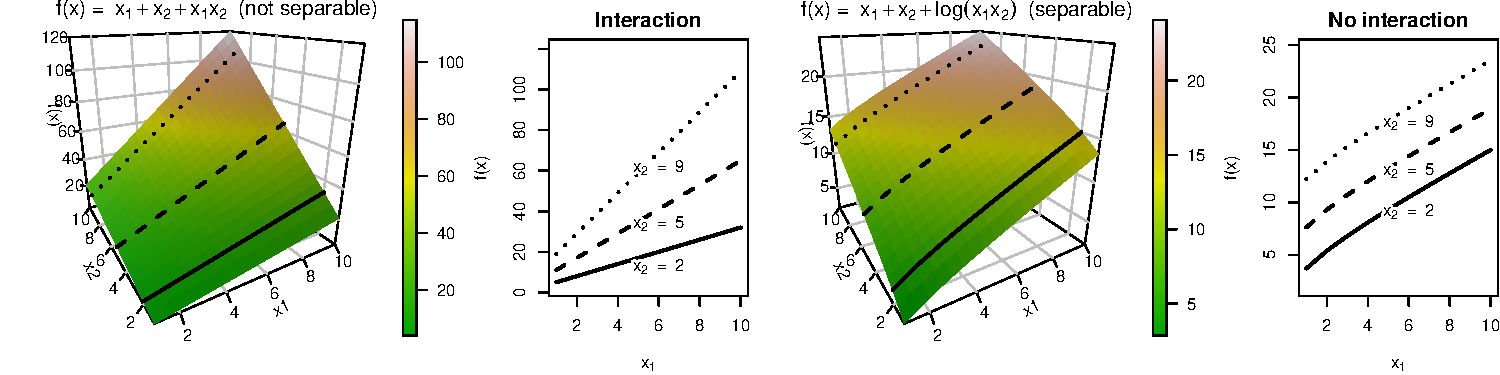
\includegraphics[width = 0.8\textwidth, trim={0cm 0cm 0cm 0cm}, clip]{figure/interaction_separable_2}

The mean-centered ICE curve for obs. $\xv$ evaluated at $m$ grid points $\tilde x_j^{(1)}, \dots, \tilde x_j^{(m)}$ is:

{\color{cice}
\centerline{$\hat f^c(\tilde x_j, \xv_{-j}) = \hat{f}(\tilde x_j, \xv_{-j}) - \frac{1}{m} \sum\nolimits_{k=1}^m \hat{f}(\tilde x_j^{(k)}, \xv_{-j})$}}
 %and $g \in \{1,...,G\}$

\begin{columns}
    \begin{column}{0.39\textwidth}
        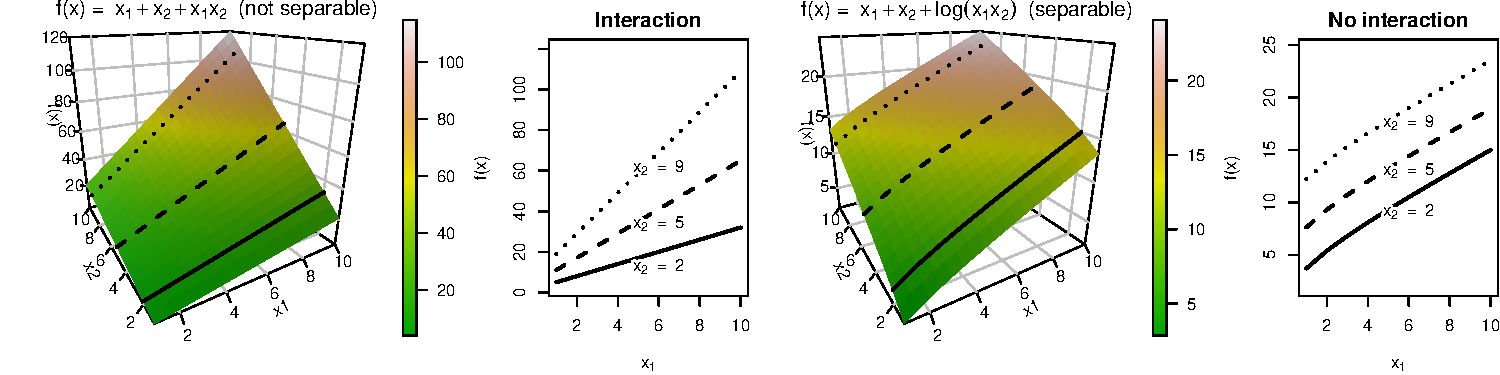
\includegraphics[width = \textwidth, trim={13cm 0cm 0cm 0cm}, clip]{figure/interaction_separable_2}
    \end{column}
    \begin{column}{0.61\textwidth}
        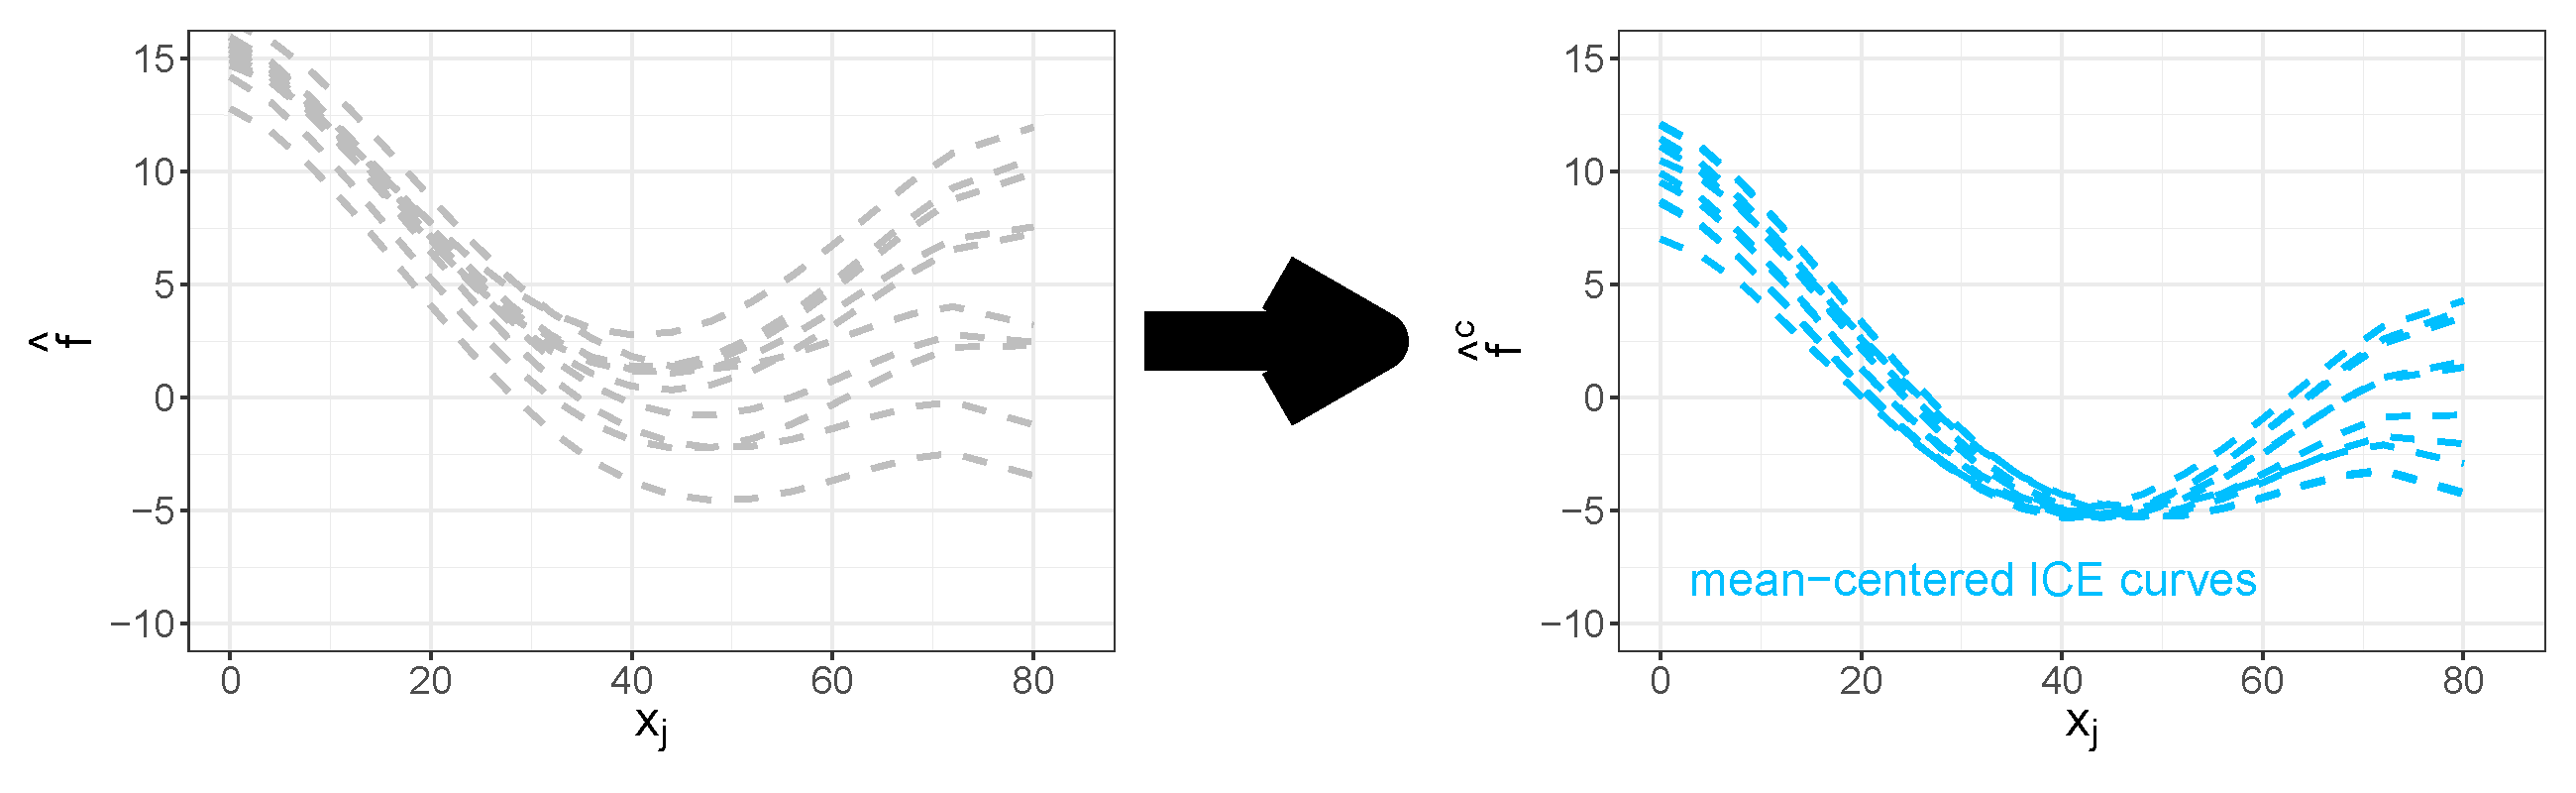
\includegraphics[width = \textwidth]{figure/ice_rep_distance0.png} 
    \end{column}
\end{columns}

%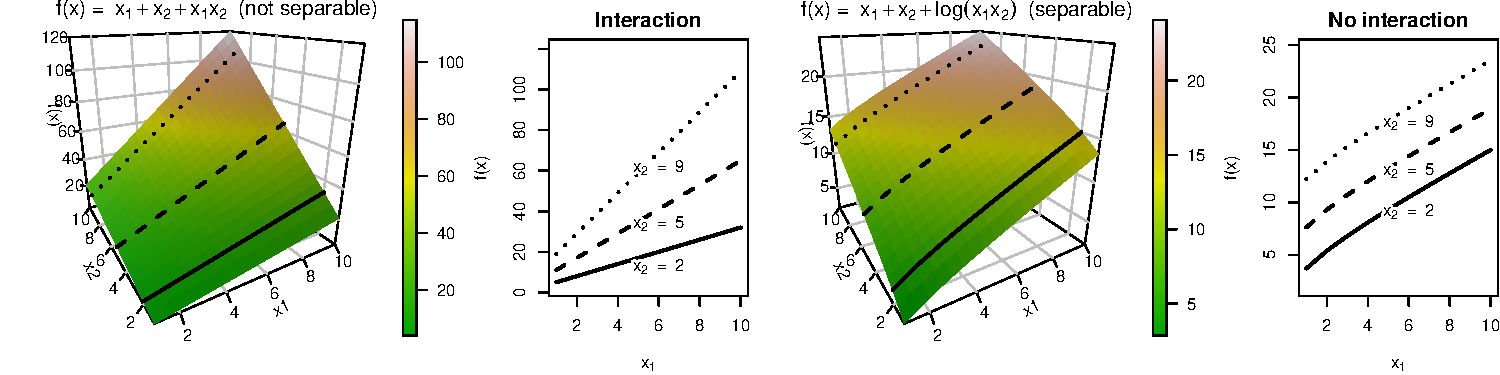
\includegraphics[width = 0.3\textwidth, trim={13cm 0cm 0cm 0cm}, clip]{figure/interaction_separable_2}
\end{frame}






\begin{frame}{Regional Effect Plots - Synthetic Example}

   
%\textbf{How can we use ICE curves to find regions with representative PDPs?}
%\vspace*{0.3cm}

\begin{columns}[T, totalwidth = \linewidth]
    \begin{column}{0.42\textwidth}


\textbf{Example:}
%$X_1, X_2 \sim \mathcal{U}(-1,1), X_3, X_5 \sim \mathcal{B}(n, 0.5), X_4 \sim \mathcal{B}(n, 0.7), X_6 \sim \mathcal{N}(1,5)$ (all iid)\\
$X_1, X_2, X_6 \sim \mathcal{U}(-1,1)$, 
$X_3, X_4, X_5 \sim \mathcal{B}(n, 0.5)$ (all iid)\\

%$\leadsto$ True relationship: $f(X) = 0.2 X_1 - 8 X_2 + \color{YellowGreen}{8 X_2  \mathbbm{1}_{(X_1 > 0)}} \color{black}+ \color{ForestGreen}{16 X_2  \mathbbm{1}_{(X_3 = 0)}} \color{black}+ \epsilon, \; \epsilon \sim \mathcal{N}(0,1)$\\

$\leadsto$ Model: Random forest

        \begin{itemize}
  %\setlength{\itemindent}{0em}
\item \textbf{Problem:} 
\begin{itemize}
    \item \only<1>{PD curve of $\highlight{X_2}$ is misleading due to interactions $\leadsto$ ICE}
    \only<2->{PD curve of $X_2$ is misleading due to interactions $\leadsto$ ICE}
    \item ICE curves do not identify the interacting features
\end{itemize}


\item<2-> \textbf{Idea:} Find regions with similar ICE curves and aggregate them to regional effects
% \item<2-> \textbf{Idea:} Find regions where variance of ICE curves is minimized by recursive partitioning the feature space w.r.t. all other features $-j$\\
%Find regions with similar ICE curves and aggregate them to regional effects\\
%\item 
%$\leadsto$ REP more representative due to less interactions  
   %\item[$\leadsto$]\textbf{Idea} Recursively partition feature space w.r.t. $-j$ such that distance of ICE curves to REP is small}
\item<3-> {\color{rep}\textbf{Regional effect}} (blue curves)   $\hat = $ Estimate PD curve in each region

 % \centerline{$ \textstyle    \hat f_{j|\mathcal{N}_g}^{PD}(\tilde x_j) = \frac{1}{|\mathcal{N}_g|} \sum_{i \in \mathcal{N}_g} \hat f(\tilde x_j, \xv_{-j}^{(i)})$}
\end{itemize}


   
    \end{column}
    \begin{column}{0.55\textwidth}
    \small
    \only<1>{\centerline{
    $f(X) = 0.2 X_1 \highlight{- 8 X_2 + {8 X_2  \mathbbm{1}_{(X_1 > 0)}}+ {16 X_2  \mathbbm{1}_{(X_3 = 0)}}} + \epsilon $}}
    \only<2>{\centerline{
    $f(X) = 0.2 X_1 - 8 X_2 + {8 X_2  \mathbbm{1}_{(X_1 > 0)}} + \highlightFG{16 X_2  \mathbbm{1}_{(X_3 = 0)}} \color{black}+ \epsilon $}}
    \only<3>{\centerline{
    $f(X) = 0.2 X_1 - 8 X_2 + \highlightYG{8 X_2  \mathbbm{1}_{(X_1 > 0)}} \color{black}+ \highlightFG{16 X_2  \mathbbm{1}_{(X_3 = 0)}} \color{black}+ \epsilon $}}
    %$, \; \epsilon \sim \mathcal{N}(0,1)$
\only<1>{
    \centering
      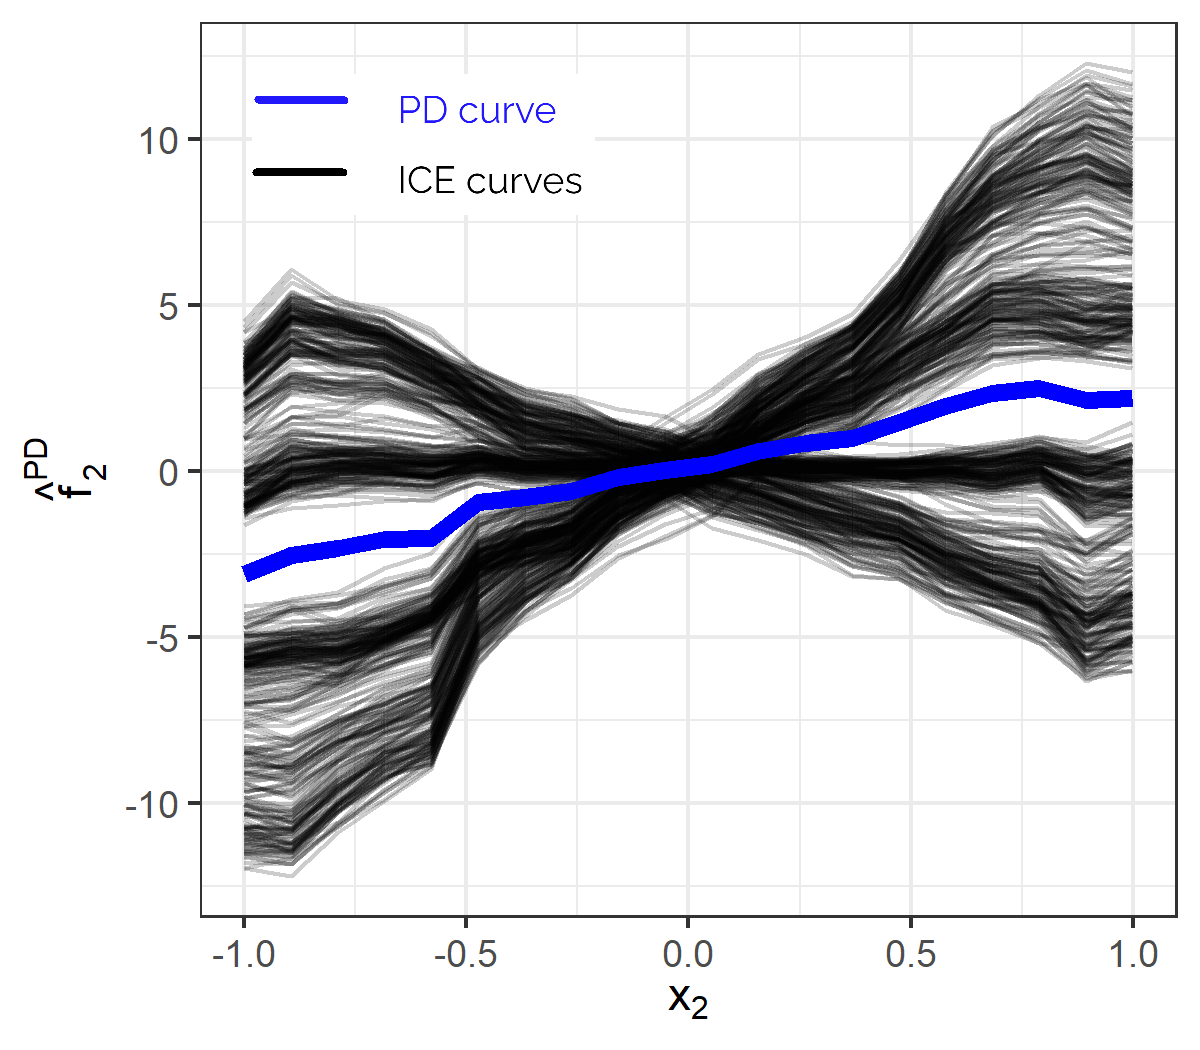
\includegraphics[width=0.82\textwidth]{figure/sim1_allcurves.png} 
}
\only<2->{
\centering
     %\begin{minipage}[t]{.5\textwidth}
     \hspace{-20pt}
     \includegraphics<2>[width=0.5\textwidth]{figure/sim1_allcurves.png}
     
     \only<2>{
           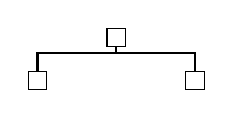
\begin{tikzpicture}
      \usetikzlibrary{arrows}
        \usetikzlibrary{shapes}
         \tikzset{treenode/.style={draw}}
         \tikzset{line/.style={draw, thick}}
     % Nodes
    \node [treenode] (a0) {}; [below=1pt,at=(10,0)]  {};% Top node
    \node [treenode, below=0.3cm of a0, xshift=-1.0cm] (a1) {}; % Bottom left node
    \node [treenode, below=0.3cm of a0, xshift=1.0cm] (a2) {}; % Bottom right node

    % Lines
    \draw [thick] (a0) -- ++(0, -0.2cm) -| (a1);
    \draw [thick] (a0) -- ++(0, -0.2cm) -| (a2);
      \end{tikzpicture}
     }
     
      %\fcolorbox{ForestGreen}{white}     {
      \highlightFG{
      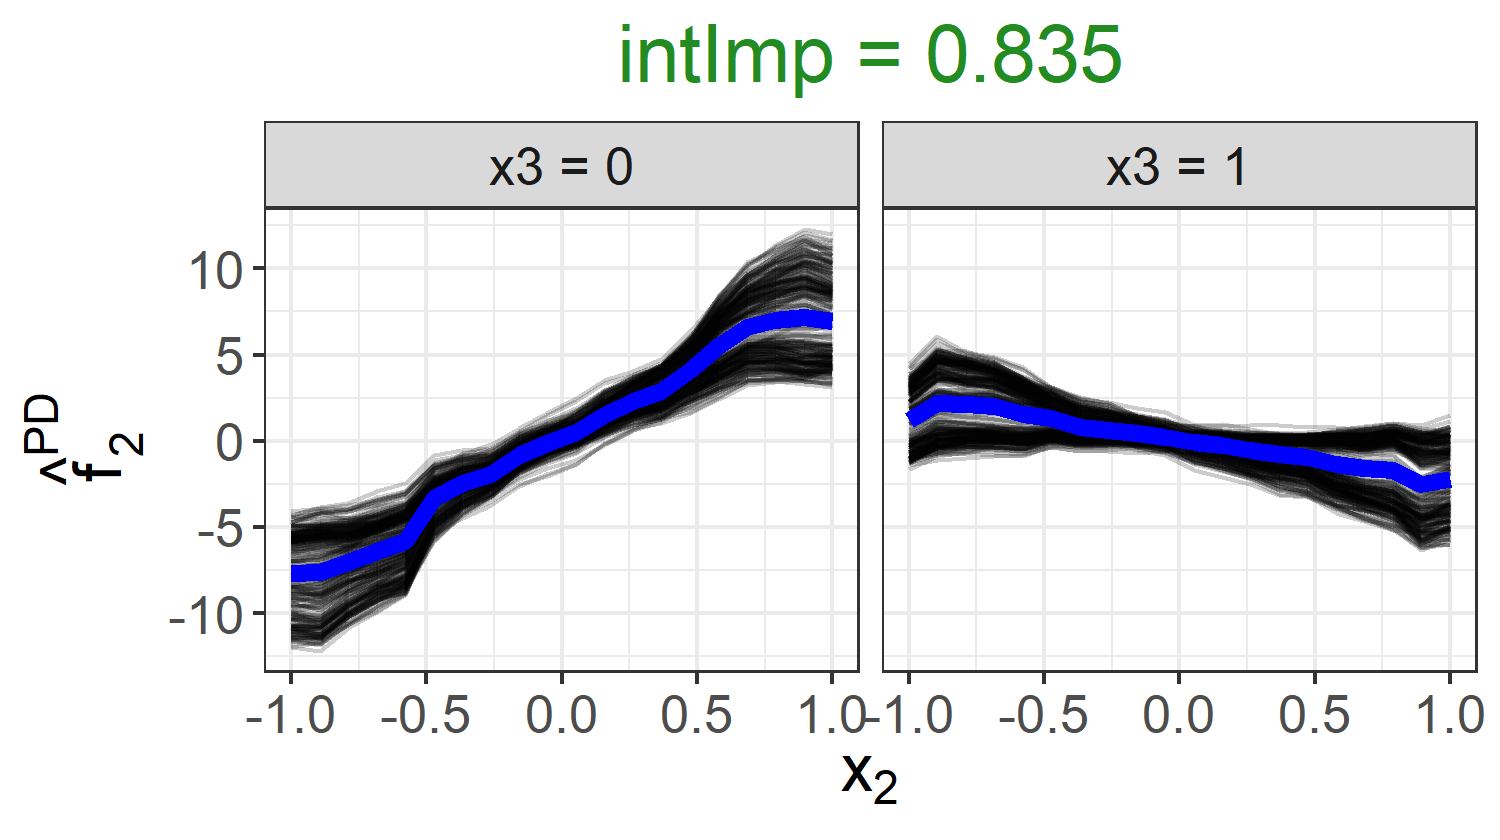
\includegraphics[width=0.6\textwidth, trim = 0 0 0 25, clip]{figure/sim1_dt_split1.png}
      }
      %}
}
\only<3->{
      \scalebox{1}{
      \hspace{15pt} 
      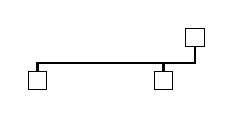
\begin{tikzpicture}
      \usetikzlibrary{arrows}
        \usetikzlibrary{shapes}
         \tikzset{treenode/.style={draw}}
         \tikzset{line/.style={draw, thick}}
        \node [treenode](a0) {} ; [below=1pt,at=(4,0)]  {};
         \node [treenode, below=0.3cm, at=(a0.south), xshift=-2.0cm]  (a1) {};
         \node [treenode, below=0.3cm, at=(a0.south), xshift=-0.4cm]  (a2) {};
         \path [line] (a0.south) -- + (0,-0.2cm) -| (a1.north) node [midway, above] {};
         \path [line] (a0.south) -- +(0,-0.2cm) -|  (a2.north) node [midway, above] {};
      \end{tikzpicture}
      \hspace{35pt}
      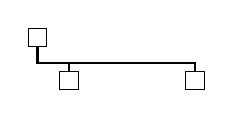
\begin{tikzpicture}
      \usetikzlibrary{arrows}
        \usetikzlibrary{shapes}
         \tikzset{treenode/.style={draw}}
         \tikzset{line/.style={draw, thick}}
        \node [treenode] (a01) {};[below=5pt,at=(node1.south) , xshift=3.5cm]
         \node [treenode, below=0.3cm, at=(a01.south), xshift=0.4cm]  (a1) {};
         \node [treenode, below=0.3cm, at=(a01.south), xshift=2.0cm]  (a2) {};
         \path [line] (a01.south) -- + (0,-0.2cm) -| (a1.north) node [midway, above] {};
         \path [line] (a01.south) -- +(0,-0.2cm) -|  (a2.north) node [midway, above] {};
      \end{tikzpicture}
      }
    %\fcolorbox{YellowGreen}{white}{
    \highlightYG{
    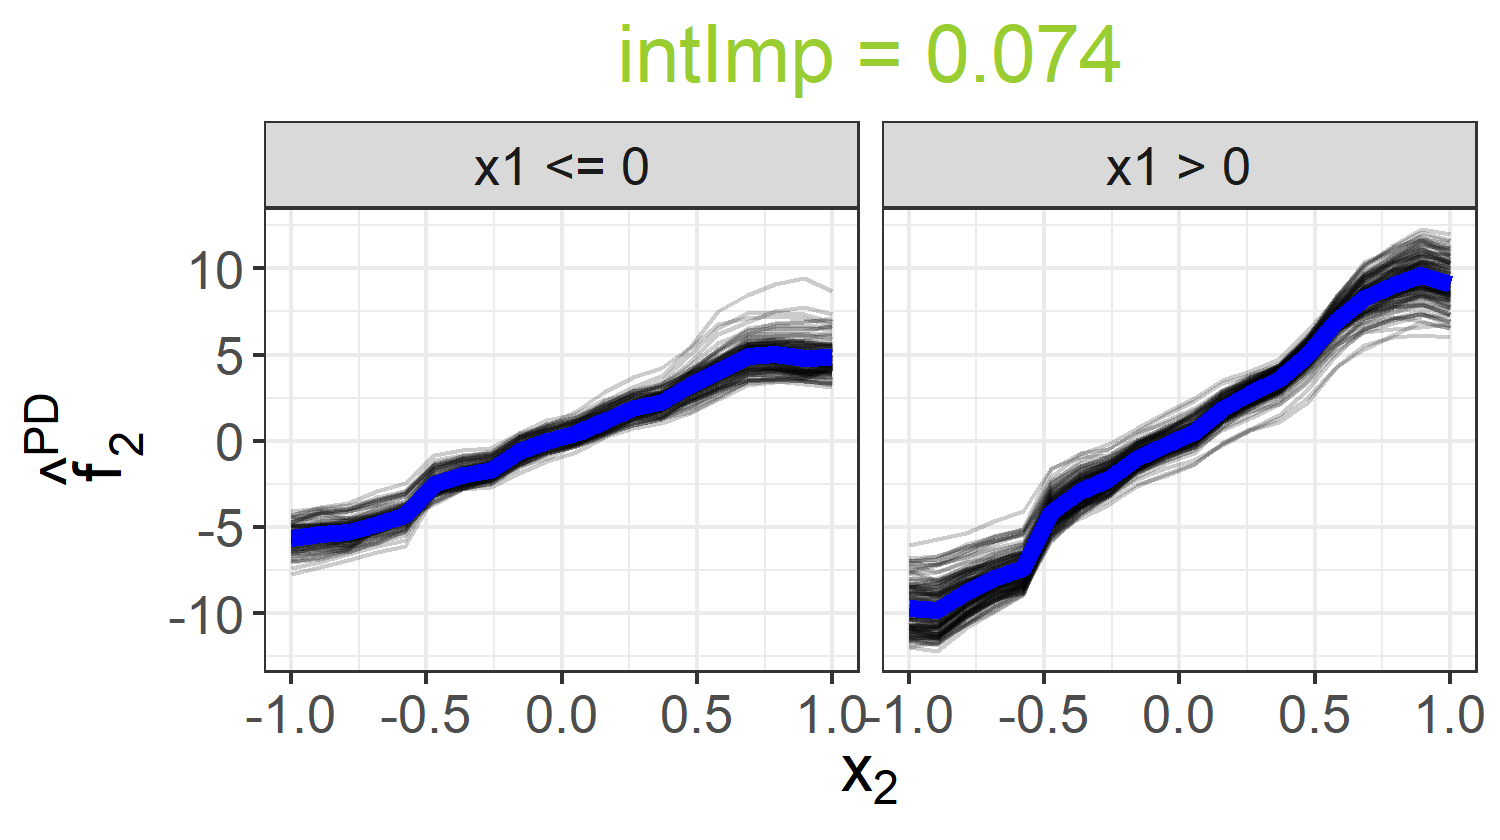
\includegraphics[width=0.52\textwidth, trim = 0 0 0 25, clip]{figure/sim1_dt_split2_1.png}
    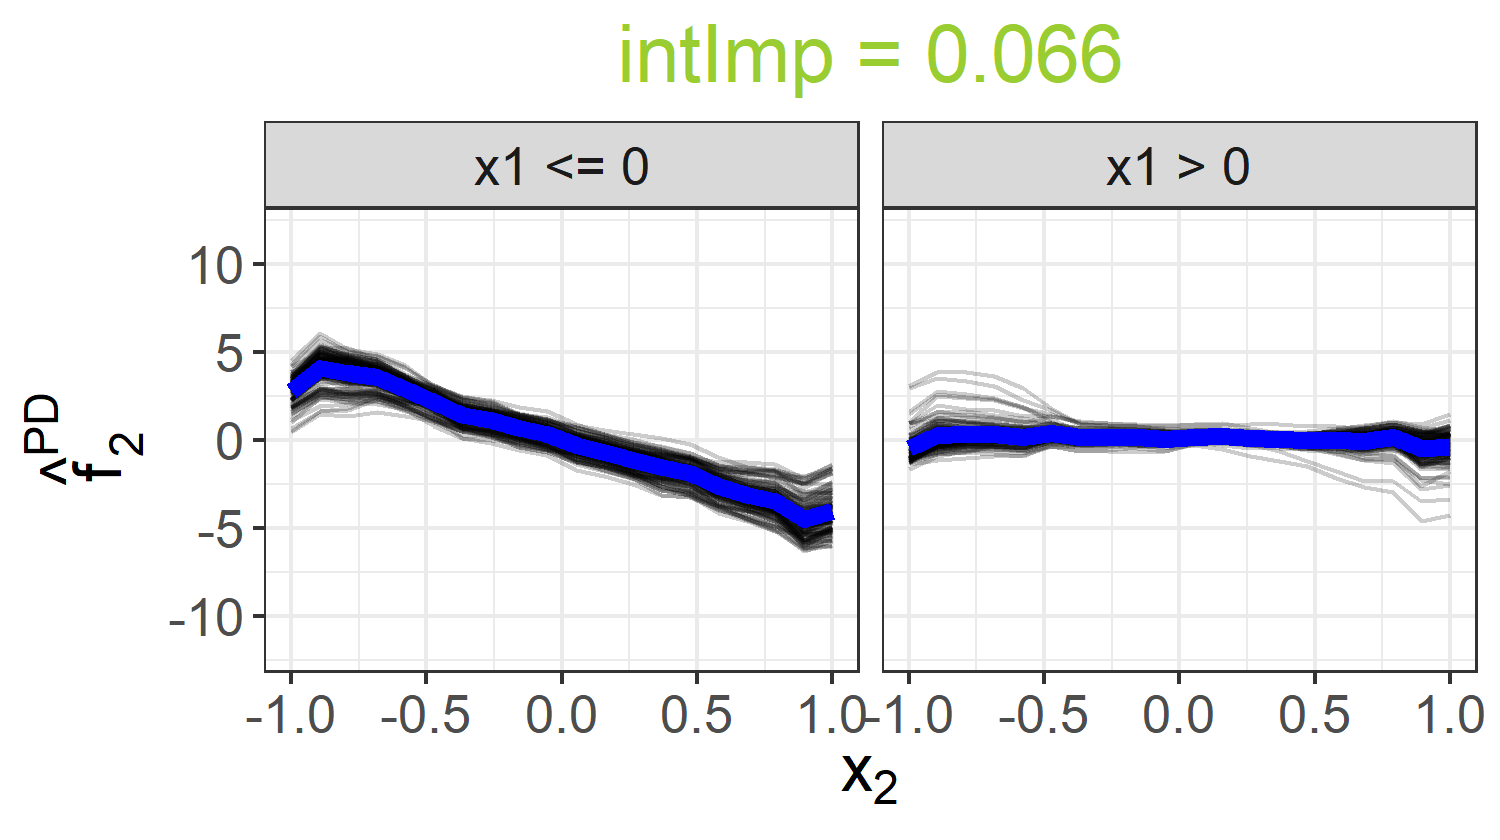
\includegraphics[width=0.46\textwidth, trim = 40 0 0 25, clip]{figure/sim1_dt_split2_2.png}
    }
    %\vspace{.2in}
    %\caption{ICE curves for $\xv_2$ are grouped by REPID and REPs (blue) are illustrated. %The first split divides the ICE curves depending on $x_3$. The second level divides the ICE curves of each child node again into two sub-regions with respect to $x_1$.
    %}
    %\label{fig:sim1_dt}
     %\end{minipage} 

     \begin{columns}[T, totalwidth = \linewidth]
     %\footnotesize
            \begin{column}{0.1\linewidth}
            \centering
             $\hat{f}_2^{PD}(X_2)$ %, X_1 > 0 \land X_3 = 0\)\\
         \end{column}
         \begin{column}{0.18\linewidth}
         \centering
             $\approx 8X_2$ %, X_1 > 0 \land X_3 = 0\)\\
         \end{column}
        \begin{column}{0.2\linewidth}
\centering
            $\approx 16X_2$ %, X_1 \leq 0 \land X_3 = 0\)
         \end{column}
        \begin{column}{0.2\linewidth}
        \centering
            $ \approx -8X_2$ %, X_1 \leq 0 \land X_3 \neq 0\)
         \end{column}        
         \begin{column}{0.2\linewidth}
         \centering
             $\approx 0$%, X_1 > 0 \land X_3 \neq 0\)\\
         \end{column}
     \end{columns}
     \medskip
     $\Rightarrow$ Additive decomposition of global feature effect
     %$f_2(X_2) \approx \sum_{i: \textit{terminal node indices}} g_i(X_2) \mathbbm{1}_{(X \in \mathcal{N}_i)}$
}


    \end{column}

\end{columns}

% \begin{minipage}[htb]{0.48\linewidth}
% \begin{itemize}

% \item \textbf{Problem:} PD plot (average of ICE) misleading

% \item \textbf{Idea:} Find regions where ICE curves are similar in their shape\\
% $\leadsto$ These regions have little interactions 

%     %\item<1-2> Grouping homogeneous ICE curves reduces individual interaction effects
%     %\item<2> REP = group marginal effect for feature of interest $x_j$ in specific region
  
% \end{itemize}
% \end{minipage}
% \only<1>{
% \begin{minipage}[htb]{0.5\linewidth}
%     \centering
%      %\begin{minipage}[t]{.5\textwidth}
%       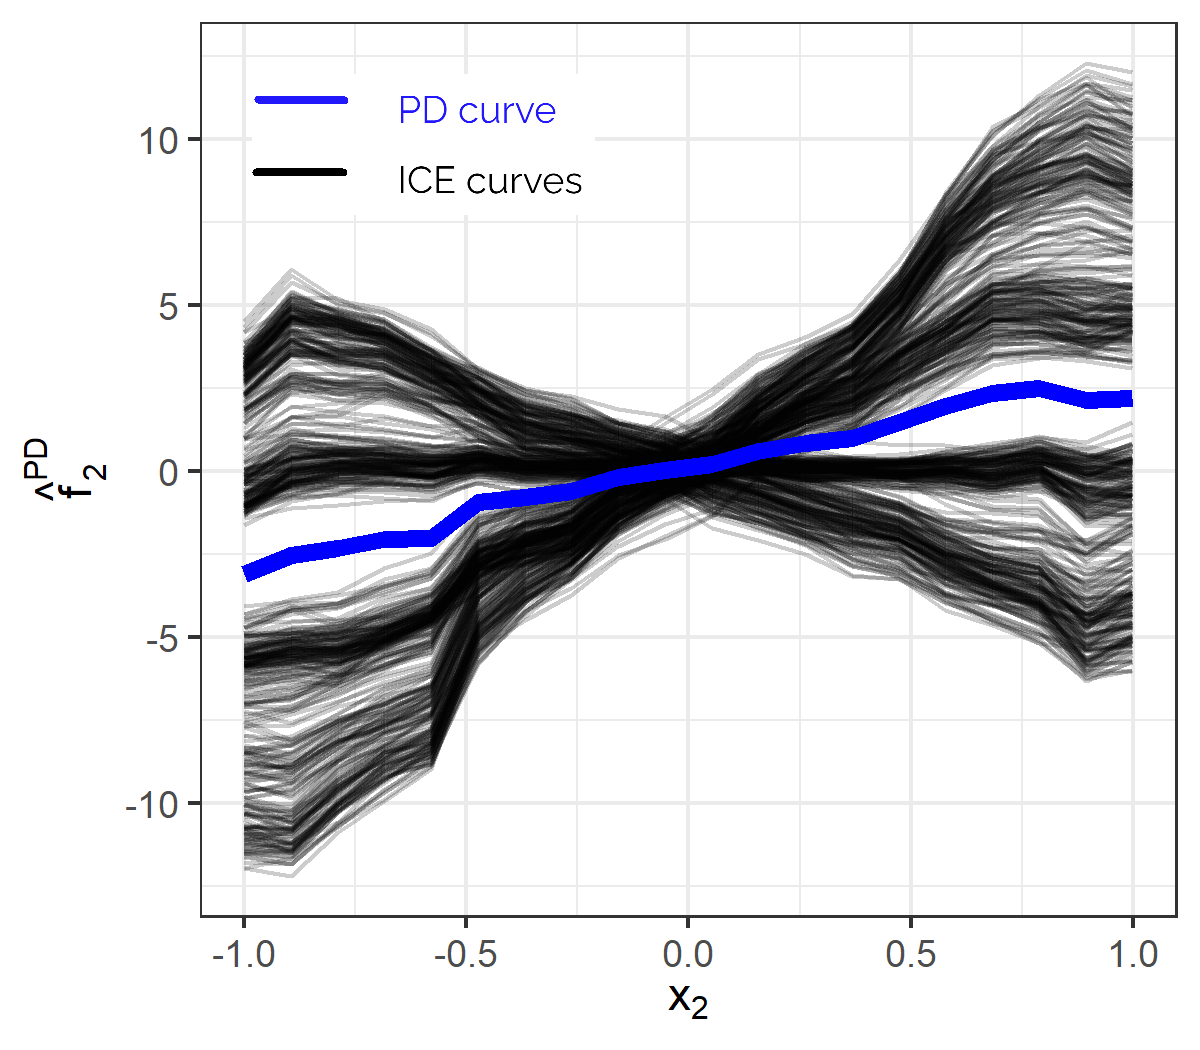
\includegraphics[width=0.9\textwidth]{figure/sim1_allcurves.png}
     
% \end{minipage}
% }
% \only<2>{
% \begin{minipage}[htb]{0.47\linewidth}
%     \centering
%      %\begin{minipage}[t]{.5\textwidth}
%       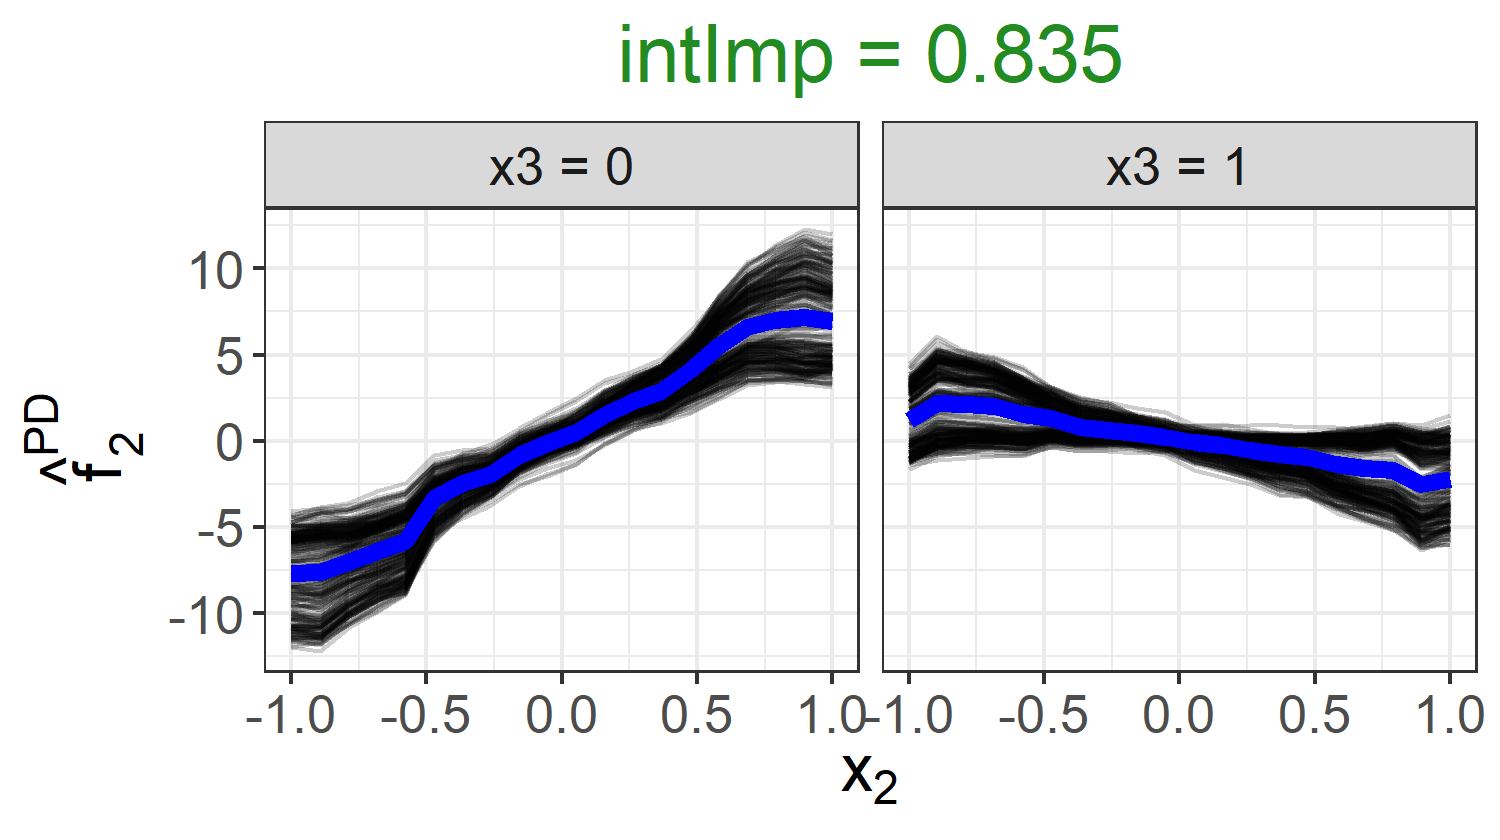
\includegraphics[width=0.49\textwidth]{figure/sim1_dt_split1.png}
%       \scalebox{1}{
%       \hspace{15pt} 
%       \begin{tikzpicture}
%       \usetikzlibrary{arrows}
%         \usetikzlibrary{shapes}
%          \tikzset{treenode/.style={draw}}
%          \tikzset{line/.style={draw, thick}}
%         \node [treenode](a0) {} ; [below=1pt,at=(4,0)]  {};
%          \node [treenode, below=0.3cm, at=(a0.south), xshift=-2.0cm]  (a1) {};
%          \node [treenode, below=0.3cm, at=(a0.south), xshift=-0.4cm]  (a2) {};
%          \path [line] (a0.south) -- + (0,-0.2cm) -| (a1.north) node [midway, above] {};
%          \path [line] (a0.south) -- +(0,-0.2cm) -|  (a2.north) node [midway, above] {};
%       \end{tikzpicture}
%       \hspace{35pt}
%       \begin{tikzpicture}
%       \usetikzlibrary{arrows}
%         \usetikzlibrary{shapes}
%          \tikzset{treenode/.style={draw}}
%          \tikzset{line/.style={draw, thick}}
%         \node [treenode] (a01) {};[below=5pt,at=(node1.south) , xshift=3.5cm]
%          \node [treenode, below=0.3cm, at=(a01.south), xshift=0.4cm]  (a1) {};
%          \node [treenode, below=0.3cm, at=(a01.south), xshift=2.0cm]  (a2) {};
%          \path [line] (a01.south) -- + (0,-0.2cm) -| (a1.north) node [midway, above] {};
%          \path [line] (a01.south) -- +(0,-0.2cm) -|  (a2.north) node [midway, above] {};
%       \end{tikzpicture}
%       }
%     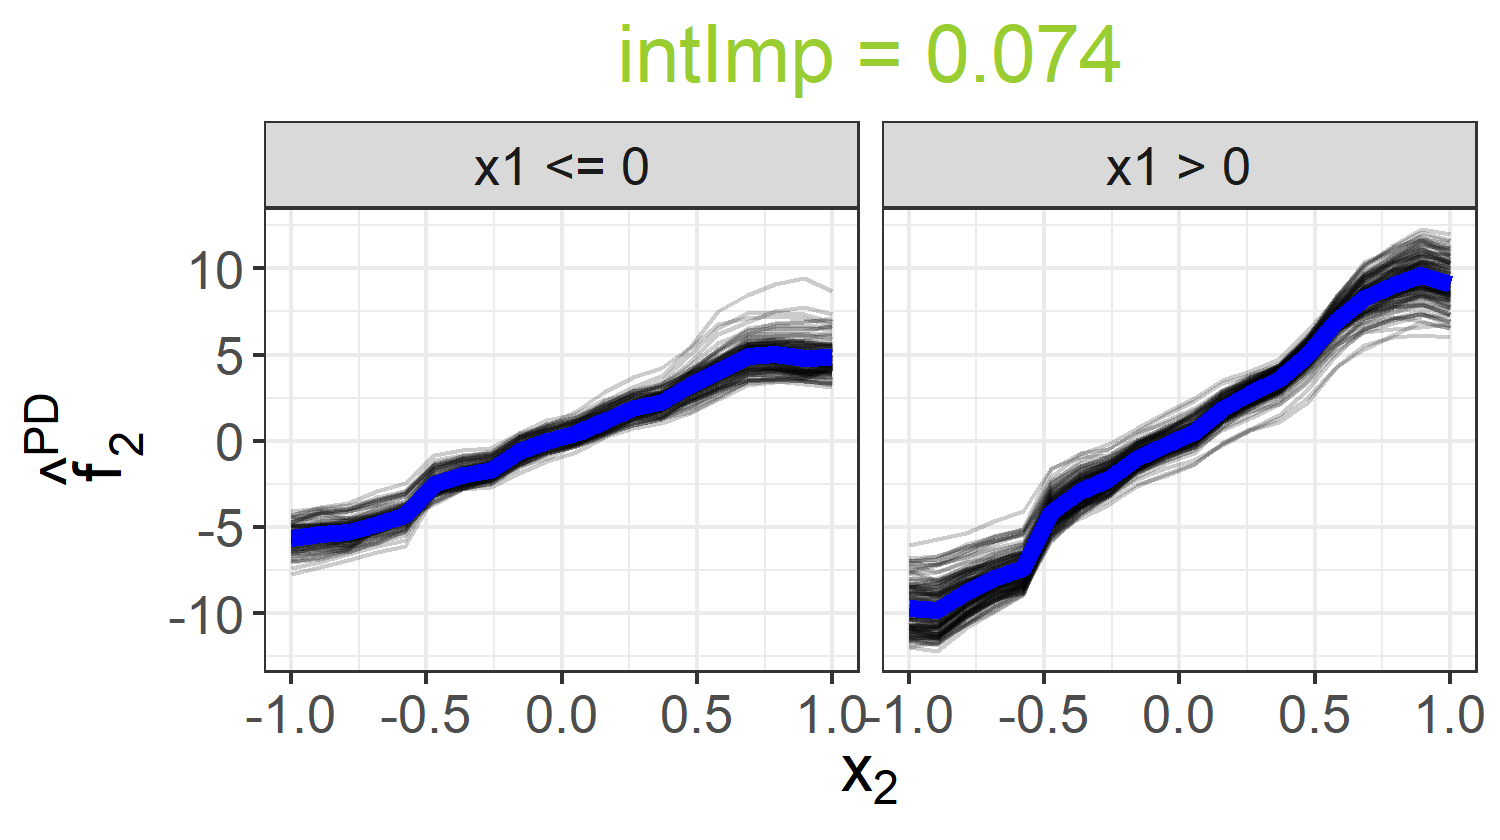
\includegraphics[width=0.49\textwidth]{figure/sim1_dt_split2_1.png}
%     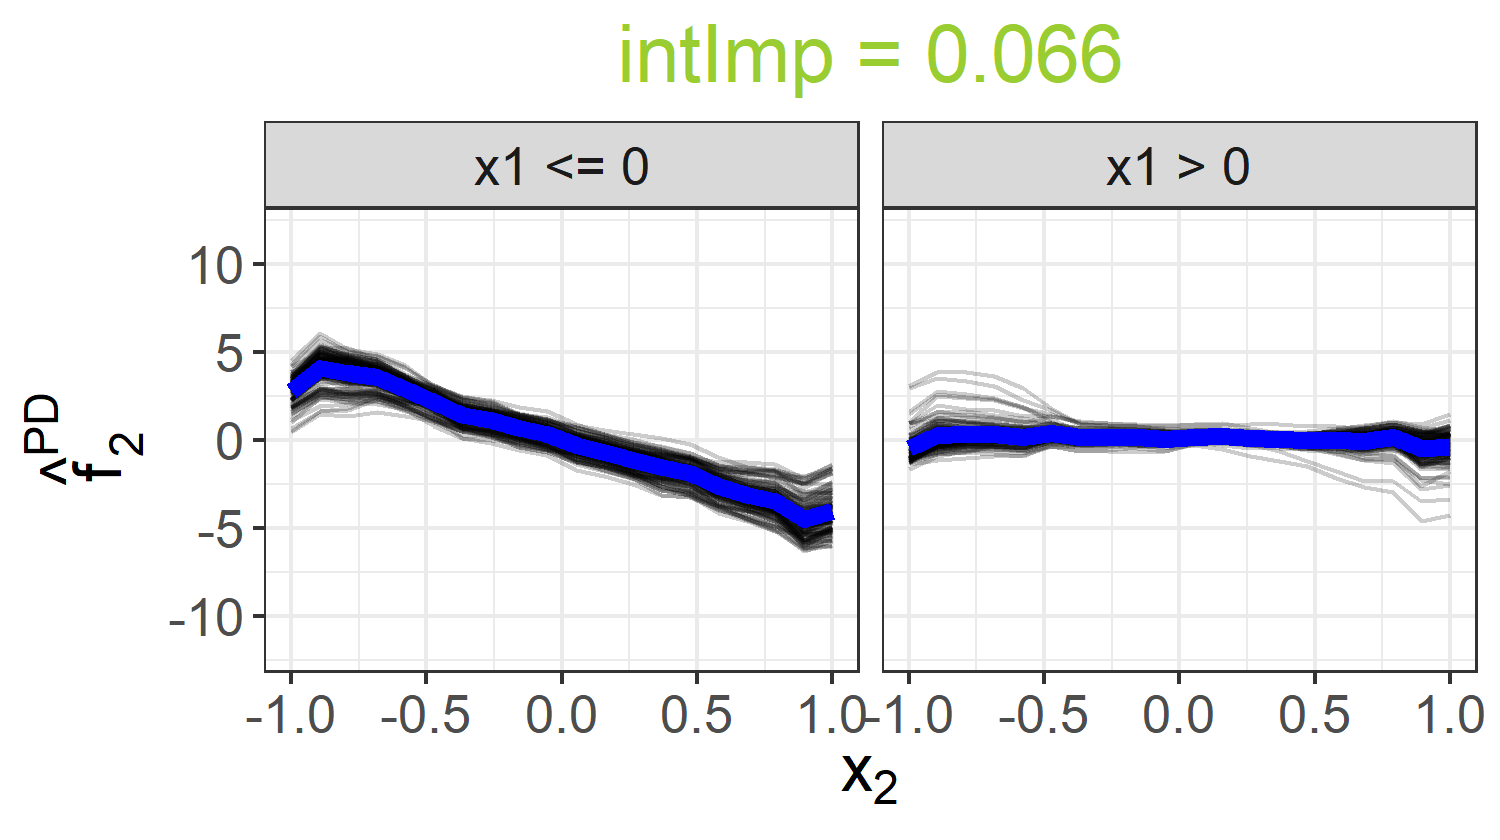
\includegraphics[width=0.49\textwidth]{figure/sim1_dt_split2_2.png}
%     \vspace{.2in}
%     %\caption{ICE curves for $\xv_2$ are grouped by REPID and REPs (blue) are illustrated. %The first split divides the ICE curves depending on $x_3$. The second level divides the ICE curves of each child node again into two sub-regions with respect to $x_1$.
%     %}
%     \label{fig:sim1_dt}
%      %\end{minipage} 
%\end{minipage}
%}


%\footnote[frame]{\textbf{AISTATS 2022:} \textit{REPID - Regional Effect Plots with implicit Interaction Detection}}

\end{frame}


\begin{frame}{Regional Effect Plots - Details}

\begin{columns}[T, totalwidth=\textwidth]
    \begin{column}{0.6\textwidth}
    \textbf{Question:} How to split the curves into regions?  
 Define risk as the L2 loss of mean-centered ICE curves:
$$\textstyle
    \mathcal{R}\left(\mathcal{N}\right) =
    \sum\limits_{\xv \in \mathcal{N}} 
     \sum\limits_{k = 1}^m
     (\underbrace{{\color{cice}\hat f^{c}(\tilde x_j^{(k)}, \xv_{-j})} - \color{rep}\hat f_{j|\mathcal{N}}^{PD,c} (\tilde x_j^{(k)})}_\text{$\color{orange}{d_k}$})^2
    %\mathcal{L}\left(\xv_j, i\right)
    $$
with the average feature effect in %region with associated index set 
region $\mathcal{N} \subseteq \Xspace$:

\medskip

{\color{rep}
\centerline{$ \displaystyle    \hat f_{j|\mathcal{N}}^{PD,c}(\tilde x_j) = \frac{1}{|\mathcal{N}|} \sum_{\xv \in \mathcal{N}} \hat f^c(\tilde x_j, \xv_{-j})$}}
    \end{column}
    \begin{column}{0.39\textwidth}
            \centering
    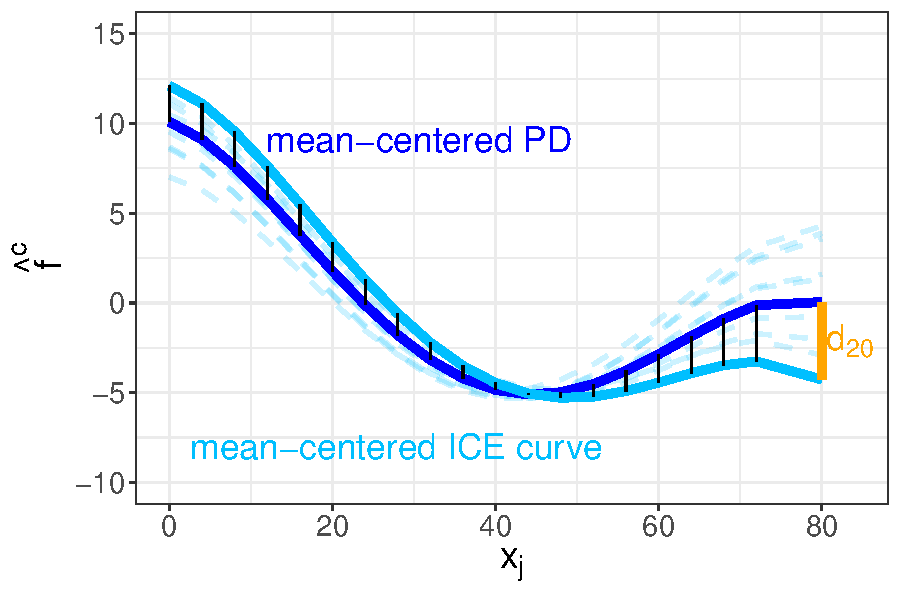
\includegraphics[width = \textwidth]{figure/ice_rep_distance2.pdf}
    \end{column}
\end{columns}
%\medskip
\begin{itemize}
    \item[$\Rightarrow$] Measures interaction-related heterogeneity (variance) ICE curves in region $\mathcal{N}$
    \item[$\Rightarrow$] Recursive partitioning (as in CART): Find the best feature-split combination that minimizes
    
% \medskip

\centerline{$\mathcal{R}\left(\mathcal{N}_{left}\right) + \mathcal{R}\left(\mathcal{N}_{right}\right)$}
\end{itemize}

      \begin{columns}[c, totalwidth=\textwidth]
        \begin{column}{0.4\textwidth}
    \begin{itemize}
        \item $\mathcal{N}_{left} = \{\xv \in \mathcal{N}|x_z \leq t\}$
        \item $\mathcal{N}_{right} = \{\xv \in \mathcal{N}|x_z > t\}$
        \item Split point $t$ for feature $x_z, z \in -j$
    \end{itemize}
        \end{column}
          \begin{column}{0.59\textwidth}
          \centering
          \textbf{Intuition:} Is another feature $x_z$ \\responsible for the heterogeneity?
        \end{column}
    \end{columns}
        %\item loss $\mathcal{L}$ for $i$-th ICE curve based on a grid of size $m$
        %\item aggregate over all ICEs within region $\mathcal{N}$
    %\end{itemize}
%\footnote[frame]{\textbf{AISTATS 2022:} \textit{REPID - Regional Effect Plots with implicit Interaction Detection}}
\end{frame}


\begin{frame}{Regional Effect Plots - Real Example}
    \begin{columns}
        % First column (Design matrix and target variable)
        \column{0.5\textwidth}
        \textbf{Dataset Overview}  % Title for the first column
        \vspace{0.5em}  % Adds a small space after the title
        \begin{itemize}
            \item Hourly count of bike-rentals (2011, 2012)
            \item Design-matrix $X$:
            \begin{itemize}
                \item Seasonal information:
                \begin{itemize}
                    \item year, month, day
                    \item hour
                    \item working day vs. non-working day
                \end{itemize}
                \item Weather information:
                \begin{itemize}
                    \item temperature
                    \item humidity
                    \item windspeed
                \end{itemize}
            \end{itemize}
            \item Target variable $Y$:
            \begin{itemize}
                \item bike-rentals per hour
                \item $Y_\mu = 189.5$, $Y_\sigma = 181.4$
            \end{itemize}
        \end{itemize}

        % Second column (ML model and explanation plots)
        \column{0.5\textwidth}
        \only<2>{
        \textbf{Modeling and Analysis}  % Title for the first column
        \vspace{0.5em}  % Adds a small space after the title
        \begin{itemize}
            \item We trained a Neural Network
            \begin{itemize}
                \item Any ML model could be used
                \item Error: $\texttt{RMSE} \approx 45.35$ counts ($0.25Y_\sigma$)
            \end{itemize}
            \vspace{0.5em} 
            
            \item Use global/regional effects to understand:
            \begin{itemize}
                \item which feature(s) are the most important
                \item how each feature affects the output
                \item which feature effects are heterogeneous 
                \item try regional effects for better explanations
            \end{itemize}
        \end{itemize}
        }
    \end{columns}
\end{frame}


\begin{frame}{Regional Effect Plots - Real Example}
\begin{figure}
    \centering
    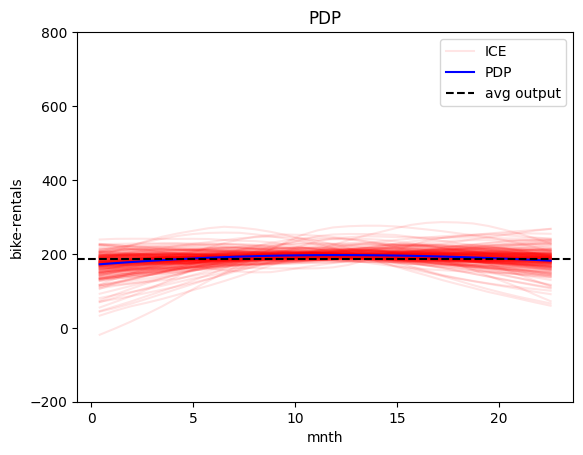
\includegraphics[width=0.3\linewidth]{figure/01_bike_sharing_dataset_18_0.png}
    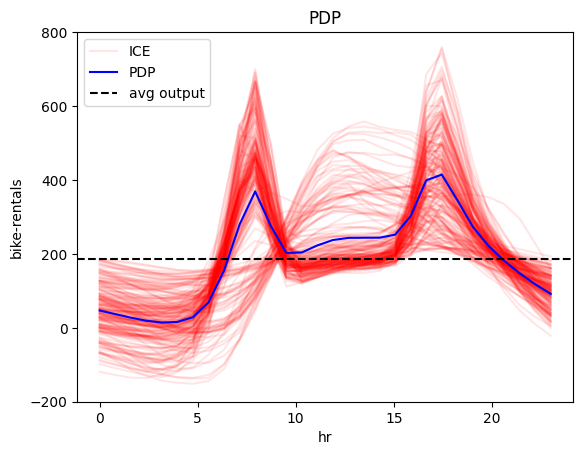
\includegraphics[width=0.3\linewidth]{figure/01_bike_sharing_dataset_18_1.png}
    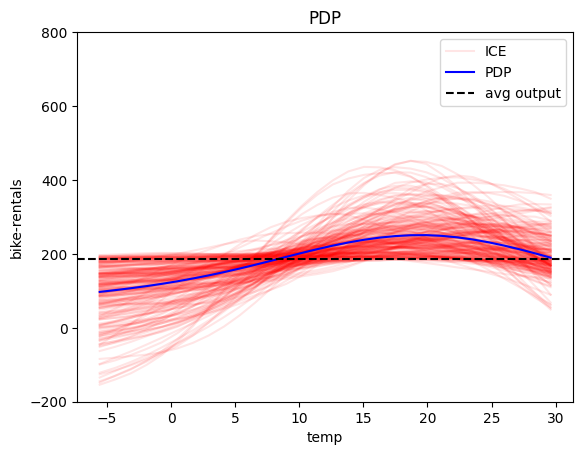
\includegraphics[width=0.3\linewidth]{figure/01_bike_sharing_dataset_18_2.png}\\
    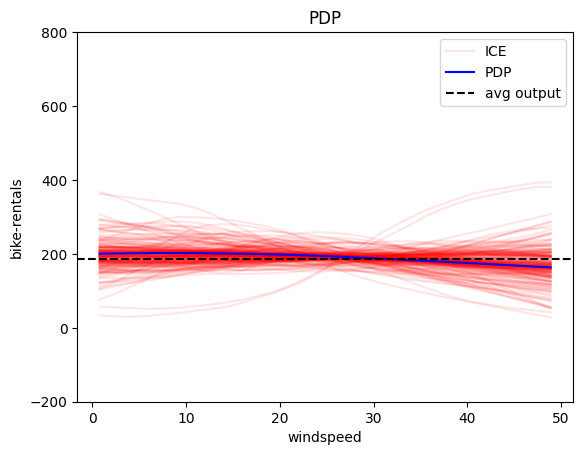
\includegraphics[width=0.3\linewidth]{figure/01_bike_sharing_dataset_18_4.png}
    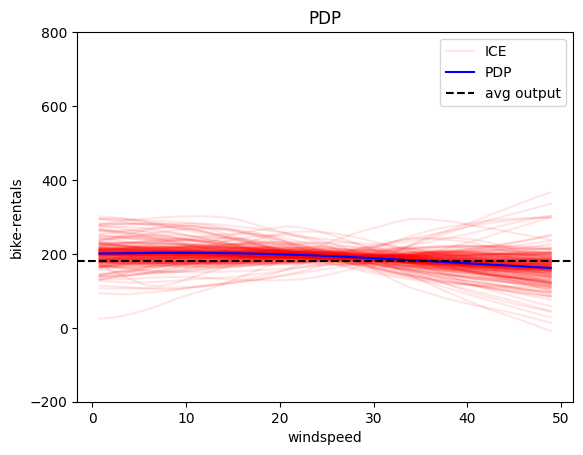
\includegraphics[width=0.3\linewidth]{figure/01_bike_sharing_dataset_18_5.png}    
    \caption{Global effect of features: month, hour, temperature, windspeed, humidity}
    \label{fig:enter-label}
\end{figure}
\begin{itemize}
    \item<2> \textcolor{ForestGreen}{\texttt{hour}: Most important and highly heterogeneous feature}
    \item<2> \texttt{temperature}: Second most important feature
    \item<2> Other features have less impact
\end{itemize}
% Now drawing the rectangle around the second image on the second slide
\only<2>{
    \begin{tikzpicture}[overlay, remember picture]
        \draw[ForestGreen, thick] (4.25, 5.7) rectangle (4.25 + 3.75, 5.7 + 3); % Adjust these coordinates
    \end{tikzpicture}
}
\end{frame}



\begin{frame}{Regional Effect Plots - Real Example}
    \centering
    \begin{tikzpicture}[every node/.style={anchor=south, align=center}]

        \node[draw, fill=yellow!20, text width=4cm] at (-4.5, 1.3) {Regional effects of \texttt{hour}};
        % Root image
        \node (root) {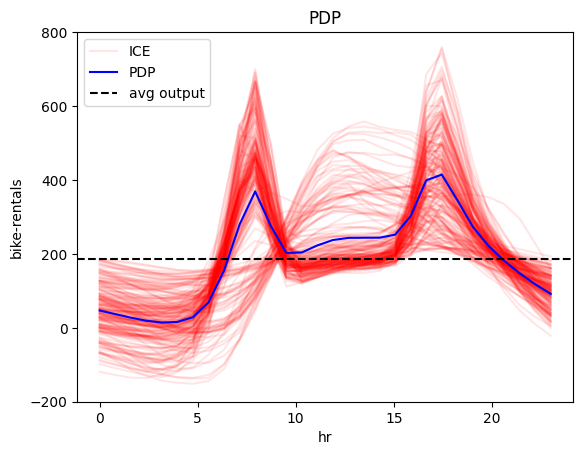
\includegraphics[width=0.25\textwidth]{figure/01_bike_sharing_dataset_18_1.png}};

        % Depth 1 (Appears on Slide 2)
        \node[below left=-.2cm and .8cm of root] (child1) {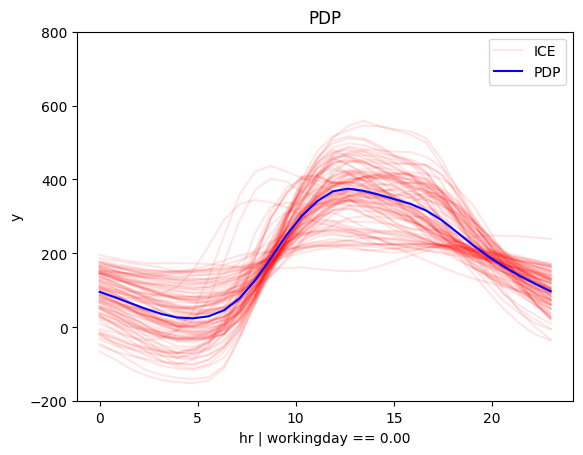
\includegraphics[width=0.25\textwidth]{figure/01_bike_sharing_dataset_28_0.png}};
        \node[below right=-.2cm and .8cm of root] (child2) {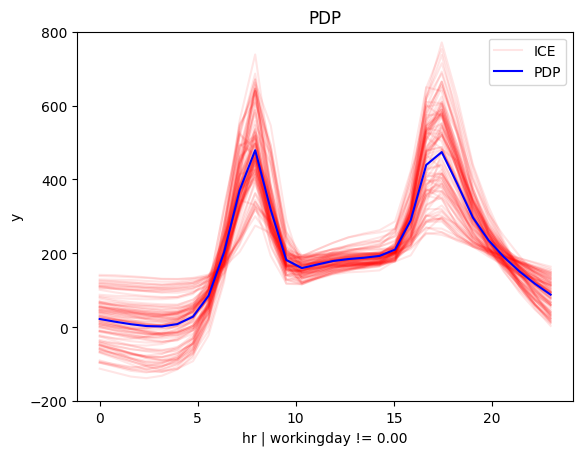
\includegraphics[width=0.25\textwidth]{figure/01_bike_sharing_dataset_28_1.png}};
        \draw (root) -- node[pos=0.15, left] {workingday=False} (child1);
        \draw (root) -- node[pos=0.15, right] {workingday=True} (child2);


        % Depth 2 (Appears on Slide 3)
        \node[below left=0.3cm and -1cm of child1] (child11) {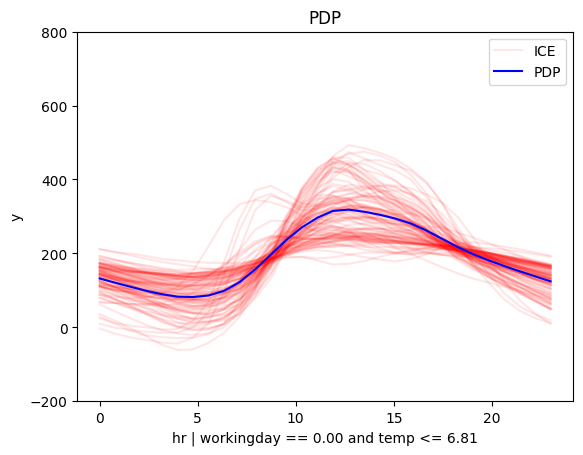
\includegraphics[width=0.25\textwidth]{figure/01_bike_sharing_dataset_29_0.png}};
        \node[below right=0.3cm and -1cm of child1] (child21) {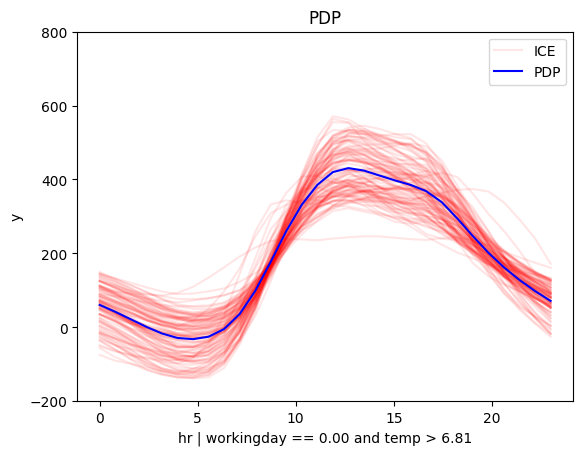
\includegraphics[width=0.25\textwidth]{figure/01_bike_sharing_dataset_29_1.png}};
        \node[below left=0.3cm and -1cm of child2] (child12) {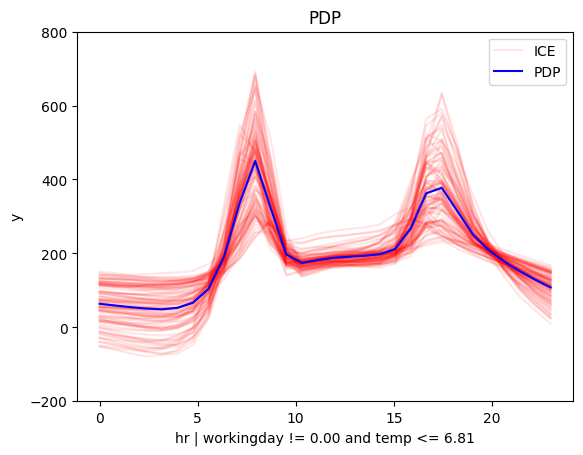
\includegraphics[width=0.25\textwidth]{figure/01_bike_sharing_dataset_29_2.png}};
        \node[below right=.3cm and -1cm of child2] (child22) {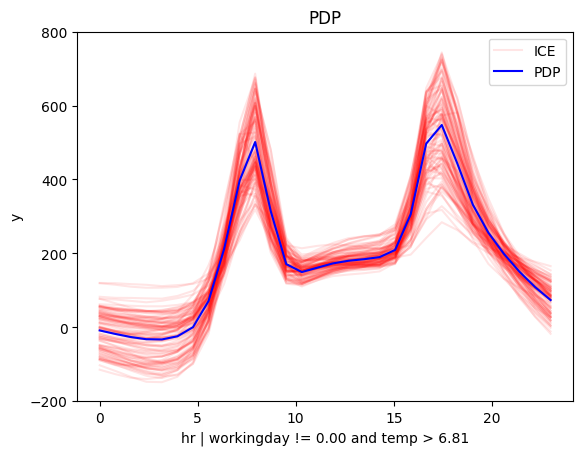
\includegraphics[width=0.25\textwidth]{figure/01_bike_sharing_dataset_29_3.png}};
        
        \draw (child1) -- node[midway, left] {temp=cold} (child11);
        \draw (child1) -- node[midway, right] {temp=hot} (child21);
        \draw (child2) -- node[midway, left] {temp=cold} (child12);
        \draw (child2) -- node[midway, right] {temp=hot} (child22);

    \end{tikzpicture}
\end{frame}


%we want to split $\mathcal{N}$ in such a way that ICE curves within the obtained regions have a similar shape meaning that the distance of these ICE curves to the REP estimate (i.e., $\hat{f}^{PD}_{S|\mathcal{N}_g} (\xv_j):= \frac{1}{|\mathcal{N}_g|}\sum_{i \in \mathcal{N}_g} \hat{f}\left(\xv_j, \xv_C^{(i)}\right)$) is small.

% \begin{frame}{Regional Effect Plots - Functional Decomposition}

% What happened?

% \end{frame}



\begin{frame}{Regional Effect Plots - \texttt{Effector}}
\begin{figure}
    
\includegraphics[width=0.5\linewidth]{figure/effector_logo.png}
    \label{fig:effector-logo}
\end{figure}
\begin{itemize}
    \item A \texttt{Python} package for global and regional effects
    \item Developed as part of the LMU-IML group
    \item Work in progress
    \begin{itemize}
        \item Keeps updating with novel methods
        \item Check future directions at the end of the presentation
    \end{itemize}
    \item \href{https://github.com/givasile/effector}{Github repo}
    \item \href{https://xai-effector.github.io/}{Documentation}

\end{itemize}
\end{frame}





\endlecture
\end{document}
